% AUTO-GENERATED durch diagram_generator (P4, Per-Achsen-Latenz-Attribution, ybar stacked)
% Ganzes je Balken = seg_run_total_ns (Wall-Clock des Segment-Laufs), NICHT total_ns (inkommensurabel,
% 3-29x daneben). Σ der 19 Segmente == seg_run_total_ns (seg_coverage~1). 18 Organ-Achsen + framework.
\begin{figure}[!htbp]
\centering
\resizebox{\textwidth}{!}{%
\begin{tikzpicture}
\definecolor{segattr0}{RGB}{230,87,87}
\definecolor{segattr1}{RGB}{179,103,68}
\definecolor{segattr2}{RGB}{230,177,87}
\definecolor{segattr3}{RGB}{179,173,68}
\definecolor{segattr4}{RGB}{192,230,87}
\definecolor{segattr5}{RGB}{114,179,68}
\definecolor{segattr6}{RGB}{102,230,87}
\definecolor{segattr7}{RGB}{68,179,91}
\definecolor{segattr8}{RGB}{87,230,162}
\definecolor{segattr9}{RGB}{68,179,161}
\definecolor{segattr10}{RGB}{87,207,230}
\definecolor{segattr11}{RGB}{68,126,179}
\definecolor{segattr12}{RGB}{87,117,230}
\definecolor{segattr13}{RGB}{79,68,179}
\definecolor{segattr14}{RGB}{147,87,230}
\definecolor{segattr15}{RGB}{149,68,179}
\definecolor{segattr16}{RGB}{230,87,222}
\definecolor{segattr17}{RGB}{179,68,138}
\definecolor{segattr18}{RGB}{230,87,132}
\begin{axis}[
    ybar stacked,
    bar width=22pt,
    width=0.7800\textwidth,
    height=0.4000\textheight,
    scale only axis,
    title={Gestapelte Per-Achsen-Latenz-Attribution},
    xlabel={Suchalgorithmus},
    ylabel={Latenz-Attribution je Achse (ns, Segment-Lauf-Wall-Clock)},
    grid=both,
    enlargelimits=0.05,
    ymin=0,
    % F-4/B: EINE Kategorie -> numerischer Index statt symbolic x coords, Fenster explizit
    xmin=-0.5, xmax=0.5,
    xtick={0},
    xticklabels={k\_ary},
    x tick label style={font=\small},
    legend style={at={(1.03,1)},anchor=north west,font=\tiny,legend cell align=left},
    reverse legend,
]
\addplot[fill=segattr0,draw=black!45,very thin] coordinates {(0,1007540.0000)};
\addlegendentry{search\_algo}
\addplot[fill=segattr1,draw=black!45,very thin] coordinates {(0,9947604.0000)};
\addlegendentry{cache\_traversal}
\addplot[fill=segattr2,draw=black!45,very thin] coordinates {(0,10423660.0000)};
\addlegendentry{mapping}
\addplot[fill=segattr3,draw=black!45,very thin] coordinates {(0,68320.0000)};
\addlegendentry{path\_compression}
\addplot[fill=segattr4,draw=black!45,very thin] coordinates {(0,47230.0000)};
\addlegendentry{node\_type}
\addplot[fill=segattr5,draw=black!45,very thin] coordinates {(0,45630.0000)};
\addlegendentry{memory\_layout}
\addplot[fill=segattr6,draw=black!45,very thin] coordinates {(0,220.0000)};
\addlegendentry{allocator}
\addplot[fill=segattr7,draw=black!45,very thin] coordinates {(0,1019670.0000)};
\addlegendentry{prefetch}
\addplot[fill=segattr8,draw=black!45,very thin] coordinates {(0,43840.0000)};
\addlegendentry{concurrency}
\addplot[fill=segattr9,draw=black!45,very thin] coordinates {(0,11870.0000)};
\addlegendentry{serialization}
\addplot[fill=segattr10,draw=black!45,very thin] coordinates {(0,12450.0000)};
\addlegendentry{value\_handle}
\addplot[fill=segattr11,draw=black!45,very thin] coordinates {(0,17041.0000)};
\addlegendentry{index\_organization}
\addplot[fill=segattr12,draw=black!45,very thin] coordinates {(0,11600.0000)};
\addlegendentry{io\_dispatch}
\addplot[fill=segattr13,draw=black!45,very thin] coordinates {(0,1910.0000)};
\addlegendentry{migration\_policy}
\addplot[fill=segattr14,draw=black!45,very thin] coordinates {(0,73394.0000)};
\addlegendentry{filter}
\addplot[fill=segattr15,draw=black!45,very thin] coordinates {(0,8910.0000)};
\addlegendentry{queuing\_q1}
\addplot[fill=segattr16,draw=black!45,very thin] coordinates {(0,74210.0000)};
\addlegendentry{queuing\_q2}
\addplot[fill=segattr17,draw=black!45,very thin] coordinates {(0,140.0000)};
\addlegendentry{persistence\_target}
\addplot[fill=segattr18,draw=black!45,very thin] coordinates {(0,3580.0000)};
\addlegendentry{framework}
\end{axis}
\end{tikzpicture}
}%
\caption{Gestapelte Per-Achsen-Latenz-Attribution}
\end{figure}
